\documentclass[10pt]{article}
\usepackage{fullpage}
\usepackage{tikz}

\usetikzlibrary{shapes.geometric, arrows}

\tikzstyle{file} = [rectangle, rounded corners, minimum width=3cm, minimum height=1cm, text centered, text width=3cm, draw=black]
\tikzstyle{fileL} = [rectangle, rounded corners, minimum width=3cm, minimum height=1cm, text centered, text width=4cm, draw=black]
\tikzstyle{folder} = [rectangle, minimum width=3cm, minimum height=1cm, text centered, text width=3cm, draw=black]
\tikzstyle{arrow} = [thick, ->, >=stealth]

\begin{document}

\title{\vspace{-2cm}ARM Checkpoint - Group 16}
\author{\small Ayoob Ahmed, Aayush Dalal, Al-Maz Ahmad, Devam Savjani}


\maketitle

This report describes how we are working in a group and how we have gone about the ARM11 emulator. Working in group has proven difficult considering we cannot meet in person however we have been able to mitigate this problem by using various online platforms including Whatsapp and Discord.
\section{Group Organisation}
\subsection{Delegation of Workload}
In order to split the workload evenly and achieve a solution efficiently, we initially discussed how we could go about the task. We debated on particular approaches we could take, eventually agreeing on one. From that initial meeting, we each took away something to do and then split the workload in terms of functions that we would need to implement. To begin with, we considered the data types that we would need to implement, and accepted the fact that we may need to reconsider this as the project continues. 
\\As there were 4 types of instructions, we split them between each of us. We were aware of the fact that some types would require more work than others and thus, we decided that the people working on the shorter instructions (e.g. branch) would assist those working on the longer ones (e.g. Data processing) as soon as they were finished. We constantly used (and still use) our Whatsapp group-chat and frequently speak on Discord to review our tasks. Having the Discord server helps us keep track of the tasks yet to be completed , the tasks already completed as well as the status of an incomplete task. This was very useful while delegating the work in an even manner.
\subsection{The Group Dynamic}
In terms of our group dynamic and how we are working in a team, we think our team is working extremely well. We are constantly communicating on the whereabouts of each of our sub-tasks. Although even after some planning, we got off to a rocky start as some of us were slightly confused and drifted apart. However, we immediately noticed that going our separate ways would not work to produce a complete and efficient code. Thus, from then on, we began to discuss on our successes and the problems we had faced on a daily basis. This allowed us to understand tasks that are left to be done. In this way, despite the slow start, we have become stronger and more efficient in working as a team. 
 The approach of talking to each other every day to update each other has helped us a lot. If someone is unsure about their task, we swap tasks between that member and another member who understands the problem in order to find a working solution efficiently. As we finished implementing all required functions, we decided to assign two people to string the implemented functions together whereas the other two began working on the second part of the project (the assembler). After splitting up into two groups, the group working on the emulator completed the debugging and testing of the code. They also combined everything together and then, went back to complete the optional task. After passing all required (and optional) tests, they attempted to make the program more efficient and get rid of any unnecessary code.
\\In the beginning of the project, we also faced another problem as, in certain periods, some members would not be able to work. To overcome this issue, we created a log type system on our discord server such that if someone would be unable to work on the project for a day, the other team members are aware of what has been done and what is yet to be completed.

\section{Implementation Strategies}
\subsection{Structure of our Emulator}
To represent our ARM system we created a struct which contains a pointer to memory, an array of type unsigned 32-bit integer of size 17. It also contains an array that assisted the pipeline by storing two booleans; one which states whether an instruction has been fetched and the other if it has been decoded. We created an {\tt{emulator\_utils}} directory which that contains the {\tt{defines.h}} file and the other helper functions to help the execution of the instruction. The structure of our emulator is as follows:

\begin{itemize}
	\item {\tt{emulate.c}} - Contains the function {\tt{main}} which reads the input binary file then passes the data onto the pipeline in order to execute the instruction. The file also uses the {\tt{emulator\_utils\textbackslash defines.h}} header which contains all of the necessary constants, libraries, data types, enums, and the decelarations of the functions that need to be used.
	\item {\tt{decodeInstr.c}} - We had decided from the beginning to have a struct containing the big-endian instruction (due to the fact that the instructions in the file are written in little-endian) and other important value. Therefore. in order to carry out this. process we implemented the decode function.
	\item {\tt{executeInstr.c}}, {\tt{executeHelper.c}} and {\tt{shiftInstruction.c}} - These three files execute the instruction where the {\tt{executeInstr.c}} file finds out the type of the instruction and then executes it with its corresponding function, found in {\tt{executeHelper.c}}. The {\tt{shiftInstruction.c}} file contains all of the types of the shifts and has their execution functions for all of them which helps the {\tt{executeHelper.c}} with the execution of the instruction.
	\item {\tt{pipeline.c}} and {\tt{output.c}} - To simulate the three-stage pipeline, we implemented a function called 'pipeline' which is found in the {\tt{pipeline.c}} file. The {\tt{output.c}} outputs the result statuses of the registers such that it prints the value of each register and the contents of any non-zero memory locations.
	
\end{itemize}


The diagram below shows the structure of the emulate file. We created a directory {\tt{emulator\_utils}} to store all of the helper functions. Within the directory, the {\tt{defines.h}} header declares all of the constants and functions.
\begin{center}

\scalebox{0.8}{
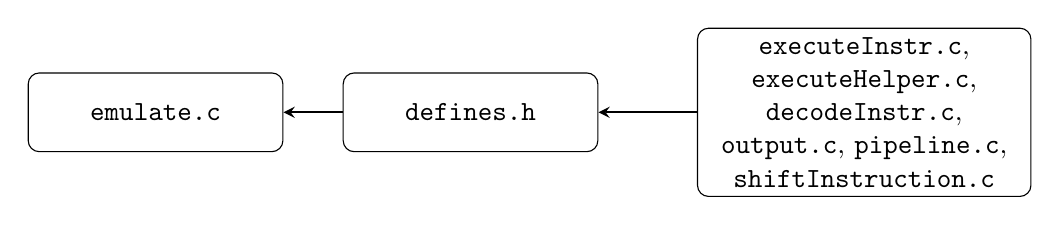
\begin{tikzpicture}[node distance=1cm]
\node (emulate) [file] {{\tt{emulate.c}}};
%\node (emulator_utils) [folder, right of=emulate, xshift=3cm] {{\tt{emulator\_utils}}};
\node (defines) [file, right of=emulate, xshift=3cm] {{\tt{defines.h}}};
\node (other) [fileL, right of=defines, xshift=4cm] {{\tt{executeInstr.c}}, {\tt{executeHelper.c}}, {\tt{decodeInstr.c}}, {\tt{output.c}}, {\tt{pipeline.c}}, {\tt{shiftInstruction.c}}};
\draw [arrow] (other) -- (defines);
\draw [arrow] (defines) -- (emulate);
%\draw [arrow] (emulator_utils) -- (emulate);
\end{tikzpicture}}
\end{center}


\subsection{The Future of our Project}
From the Emulator part, we potentially may use the endian converter to convert the instructions from big-endian to little-endian and the constants we had defined in the {\tt{defines.h}} file for the assembler. This will help in reducing the amount of magic numbers. For debugging purposes, we might also use the {\tt{output.c}} file to help us print the status of the registers as the instructions are being executed. We will have the {\tt{main}} in {\tt{assemble.c}} and we hope to structure the programs in a similar way as we structured our {\tt{emulate.c}}.
\\While discussing the second part of the project, the two members that had a head start on the assembler briefed the other two members about their ideas and some of the code they had written for reading the source file. Then, we discussed how we could implement the symbol table. Speaking about different approaches including heaps, binary trees and some others are helping us decide in the best approach we can implement, debating each of the pros and cons of each approach helped us choose an approach that would be efficient. Writing the benefits and drawbacks of each of the approaches will help us later on when implementing the ADT as we would have a clear view of the task to avoid any confusion in the task.
\\Another aspect of the task which we discussed was the tokenizer. We discussed different approaches in the same way as we did with the ADT. We conducted some more research as a group together to fill up gaps in our knowledge as a group so that we could use our research to help us work more efficiently.

\end{document}
